\documentclass[11pt,a4paper]{article}
\usepackage[utf8]{inputenc}
\usepackage[T1]{fontenc}
\usepackage[french]{babel}
\usepackage{lmodern}
\usepackage{geometry}
\geometry{top=2.5cm, bottom=2.5cm, left=2.5cm, right=2.5cm}

\usepackage{amsmath, amssymb,amsfonts}
\usepackage{graphicx}
\usepackage{booktabs}
\usepackage{xcolor}
\usepackage{hyperref}
\usepackage{circuitikz}
\usepackage{textcomp}
\usepackage{circuitikz}
\usepackage{titlesec}
\usepackage{fancyhdr}
\usepackage{subcaption}
\usepackage{pdfpages}% Requis si vous utilisez le modèle 2 (grille d'images)
\usepackage{float}       % Permet d'utiliser l'option [H] pour fixer l'image à un endroit précis
\usepackage{enumitem}    % Pour aérer les listes

% ==============================================================================
% CHARTE GRAPHIQUE ET MISE EN PAGE
% ==============================================================================
\definecolor{mainblue}{RGB}{26, 54, 93}
\definecolor{secondaryblue}{RGB}{43, 108, 176}
\definecolor{darkgray}{RGB}{45, 55, 72}
\definecolor{marron}{RGB}{128, 64, 0}
\definecolor{success}{RGB}{76,175,80}

\titleformat{\section}{\color{mainblue}\normalfont\Large\bfseries}{\thesection}{1em}{}[{\titlerule[1pt]}]
\titleformat{\subsection}{\vspace{0.5em}\color{secondaryblue}\normalfont\large\bfseries}{\thesubsection}{1em}{}
\titleformat{\subsubsection}{\vspace{0.3em}\color{darkgray}\normalfont\normalsize\bfseries\itshape}{\thesubsubsection}{1em}{}

\setlength{\parskip}{0.5em} % Espacement entre les paragraphes
\setlist{itemsep=0.3em} % Espacement dans les listes

% Configuration des liens (bleus pour rester dans la charte)
\hypersetup{colorlinks=true, linkcolor=secondaryblue, urlcolor=mainblue, citecolor=secondaryblue}

\pagestyle{fancy}
\fancyhf{}
\setlength{\headheight}{13.6pt}
\lhead{\color{darkgray}Bureau d'Étude N 3}
\rhead{\color{darkgray}Technologie MOS en Commutation}
\cfoot{\thepage}
\renewcommand{\headrulewidth}{0.4pt}

\begin{document}

% ==============================================================================
% PAGE DE GARDE
% ==============================================================================
\includepdf[pages=-]{Page_garde.pdf}

\clearpage
\tableofcontents        % Table des matières

\clearpage
\listoftables           % Liste des tableaux

\clearpage
\listoffigures          % Liste des figures

\clearpage




\newpage

% ==============================================================================
% INTRODUCTION
% ==============================================================================
\section*{Objectif du Bureau d'Étude}
\addcontentsline{toc}{section}{Objectif du Bureau d'Étude}
L'objectif est de concevoir une interface de commande basée sur un transistor MOS en mode commutation de puissance pour piloter six relais électromagnétiques \textbf{RT42405 (DC) (le lien de sa datasheet est dans les références, à la fin du document}  . Le circuit est commandé par un microcontrôleur ($3.3\text{ V}$, $20\text{ mA}$ max). L'étude se divise en deux parties : dimensionnement macroscopique avec des composants du commerce (Conception 1) et dimensionnement microscopique sur silicium en technologie ENSAT (Conception 2).

\vspace{0.5em}
\noindent \textit{\textbf{Note :}} \textit{L'intégralité des références de la nomenclature (Conception 1) a été sourcée et chiffrée via le catalogue du distributeur \href{https://www.digikey.fr/}{\textbf{DigiKey}}. }

% ==============================================================================
% CONCEPTION 1
% ==============================================================================
\section{Conception 1 : Dimensionnement et Composants}

\subsection{Question 1 : Résistances $R_1$ et $R_2$}

\subsubsection{Rôle}
\begin{itemize}
    \item \textbf{$R_1$ (Série) :} Limite le courant d'appel fourni par le microcontrôleur lors de la charge de la capacité de grille du MOSFET.
    \item \textbf{$R_2$ (Pull-down) :} Fixe le potentiel de la grille à la masse ($0\text{ V}$) en l'absence de commande, évitant les commutations intempestives.
\end{itemize}

\subsubsection{Dimensionnement théorique}
Avec $V_{OH} = 3.3\text{ V}$ et $I_{max} = 20\text{ mA}$ :
\begin{equation}
    R_{1(\text{min})} = \frac{3.3\text{ V}}{0.020\text{ A}} = 165\ \Omega \quad \Rightarrow \quad \textbf{Choix : } R_1 = 220\ \Omega
\end{equation}
Pour garantir une tension de commande suffisante, on choisit $R_2$ très supérieure à $R_1$ :
\begin{equation}
    \textbf{Choix : } R_2 = 10\ \text{k}\Omega \quad \Rightarrow \quad V_{GS} = 3.3\text{ V} \times \frac{10000}{10220} \approx 3.23\text{ V}
\end{equation}

\subsubsection{Puissances et Choix Commercial}
Le courant statique est $I \approx 0.32\text{ mA}$. La puissance de crête dissipée par $R_1$ est :
\begin{itemize}
    \item $P_{R1(\text{crête})} = \frac{V_{OH}^2}{R_1} = \frac{3.3^2}{220} = 0.0495 \text{ W} = 49.5 \text{ mW}$
    \item $P_{R2} = 10000 \times I^2 \approx 1\text{ mW}$
\end{itemize}

\textbf{Composants sélectionnés (via DigiKey) : } 

\begin{table}[H]
    \centering
    \renewcommand{\arraystretch}{1.3} 
    \resizebox{\textwidth}{!}{ 
    \begin{tabular}{|c|c|c|c|c|c|c|c|}
        \hline
        \textbf{R} & \textbf{Référence} & \textbf{Fabricant} & \textbf{Valeur} & \textbf{Tolérance} & \textbf{Puissance} & \textbf{Boîtier (Dim.)} & \textbf{Prix(min)} \\
        \hline
        R1 & RC0805FR-07220RL \cite{yageo_r220} & Yageo & 220 $\Omega$ & $\pm 1\%$ & 0,125 W & 0805 ($2.0 \times 1.25\text{mm}$) & 0,1 \$ \\
        \hline
        R2 & RC0805FR-0710KL \cite{yageo_r10k} & Yageo & 10 k$\Omega$ & $\pm 1\%$ & 0,125 W & 0805 ($2.0 \times 1.25\text{mm}$) & 0,1 \$ \\
        \hline
    \end{tabular}
    }
    \caption{Liste des composants passifs retenus}
    \label{tab:resistances}
\end{table}

\subsection{Question 2 : Transistor NMOS}

Le transistor choisi pour cette application est la référence \textbf{IRLML2502TRPbF} \cite{ir_mosfet} du fabricant International Rectifier (Infineon) en boîtier \textbf{SOT-23} (Micro3\texttrademark). 

\begin{table}[htpb]
    \centering
    \renewcommand{\arraystretch}{1.1} 
    \resizebox{\textwidth}{!}{ 
    \begin{tabular}{|c|c|p{8cm}|}
        \hline
        \textbf{Caractéristique} & \textbf{IRLML2502TRPbF \cite{ir_mosfet}} & \textbf{Justification technique} \\
        \hline
        Boîtier & CMS SOT-23 ($2.9 \times 1.3\text{mm}$) & Encombrement minimal, adapté au montage en surface. \\
        \hline
        $V_{GS(th)}$ & $0.6\text{V} - 1.2\text{V}$ & \textit{Logic-Level} : saturation totale assurée avec nos $3.23\text{V}$. \\
        \hline
        $I_D$ max & $4.2\text{ A}$ pour une $T_A= 25^\circ\text{C}$ & Très supérieur au courant de charge de la bobine ($\approx 80\text{ mA}$). \\
        \hline
        $V_{DSS}$ max & $20\text{ V}$ & Supporte largement la tension d'alimentation $V_{dd} = 5\text{V}$. \\
        \hline
        $R_{DS(on)}$ & $\le 0.080\ \Omega$ & Valeur extrêmement faible garantissant des pertes Joule négligeables. \\
        \hline
        Prix & 0,56 \$  & Composant très accessible en volume industriel.\\
        \hline
    \end{tabular}
    }
    \caption{Justifications techniques basées sur la Datasheet (DigiKey)}
    \label{tab:choix_mosfet}
\end{table}

\subsection{Question 3 : Diode de Protection}
Le rôle de cette diode, appelée diode de roue libre, est de protéger le transistor NMOS. Lors du blocage du transistor, l'inductance de la bobine s'oppose à l'annulation instantanée du courant, créant une surtension. La diode offre un chemin pour dissiper cette énergie.

\textbf{Choix commercial :} Diode de commutation rapide \textbf{6557-1N4148WTR-ND} \cite{goodwork_diode} (boîtier CMS \textbf{SOD-323}) du fabricant \textbf{GK(GOODWORK)}.

\begin{table}[htpb]
    \centering
    \renewcommand{\arraystretch}{1.3} 
    \resizebox{\textwidth}{!}{ 
    \begin{tabular}{|c|c|p{8cm}|}
        \hline
        \textbf{Caractéristique} & \textbf{6557-1N4148WTR-ND \cite{goodwork_diode}} & \textbf{Justification technique} \\
        \hline
        Boîtier & CMS SOD-323 ($1.7 \times 1.25\text{mm}$) & Ultra-compact, parfaitement adapté à l'exigence CMS. \\
        \hline
        Tension inverse ($V_{R}$) & $75\text{ V}$ & Très largement supérieure à la tension d'alimentation du relais ($V_{dd} = 5\text{ V}$). \\
        \hline
        Courant direct ($I_{F}$) & $150\text{ mA}$ & Supporte confortablement le courant de décharge de la bobine ($\approx 80\text{ mA}$). \\
        \hline
        Temps ($t_{rr}$) & $\approx 4\text{ ns}$ & Commutation extrêmement rapide, idéale pour bloquer la surtension. \\
        \hline
        Prix unitaire & $\approx 0.005\text{ \$}$ & Composant standard économique, optimisant le coût global. \\
        \hline
    \end{tabular}
    }
    \caption{Justification du choix de la diode de roue libre}
    \label{tab:choix_diode}
\end{table}
\newpage
\subsection{Schéma Électrique d'un Canal de Commande}
Ci-dessous, la structure complète implémentée pour un canal qui sera dupliqué 6 fois :

\begin{center}
\begin{circuitikz}[scale=0.85, transform shape, font=\sffamily]
    
    % --- ÉTAGE ENTRÉE : MICROCONTRÔLEUR ---
    \draw (0,0) node[anchor=east] {\scriptsize $\mu$C (3,3V)}
          to[R, l=\scriptsize $R_{in}$, a=\tiny 220$\Omega$] (1.8,0)
          to[led, l=\scriptsize LED, a=\tiny LTV-817S, *-] (1.8,-1.8) node[ground] {};
          
    % --- ÉTAGE PUISSANCE : PHOTOTRANSISTOR ---
    \draw (3.5,-0.9) node[npn, photo, scale=0.8] (opto) {};
    
    % --- BARRIÈRE D'ISOLATION GALVANIQUE ---
    \draw[dashed, gray] (1.1, 0.6) rectangle (4.1, -2.2);
    \node[gray, anchor=south] at (2.6, 0.6) {\tiny \textbf{Isolation}};
    
    % Connexion Collecteur
    \draw (opto.C) -- ++(0,0.5) node[vcc] {\tiny $V_{dd}$ 5V};
    
    % --- ÉTAGE PUISSANCE : COMMANDE DU MOSFET ---
    \draw (opto.E) |- (5.2, -1.8);
    
    % Résistance Pull-down R2
    \draw (4.5, -1.8) to[R, l=\scriptsize $R_2$, a=\tiny 10k, *-] (4.5,-3.2) node[ground] {};
    
    % Transistor MOSFET
    \draw (5.2, -1.8) node[nigfete, anchor=G, scale=0.8] (mos) {};
    \node[anchor=west, mainblue] at (mos.east) {\scriptsize \textbf{IRLML2502}}; 
    \node[anchor=south east] at (mos.G) {\tiny G};
    \node[anchor=north west] at (mos.S) {\tiny S};
    \node[anchor=south west] at (mos.D) {\tiny D};
    
    % Masse du MOSFET
    \draw (mos.S) -- ++(0,-0.5) node[ground] {};
    
    % --- ÉTAGE CHARGE : DIODE & RELAIS ---
    \draw (mos.D) -- ++(0,0.8) coordinate (D_top);
    
    % Branches parallèles réduites
    \draw (D_top) -- ++(-0.8,0) coordinate (D_left);
    \draw (D_top) -- ++(0.8,0) coordinate (D_right);
    
    % Diode de roue libre
    \draw (D_left) to[D, l=\tiny 1N4148, *-*] ++(0,1.8) coordinate (D_left_top);
    
    % Relais
    \draw (D_right) to[L, l=\tiny Relais, *-*] ++(0,1.8) coordinate (D_right_top);
    
    % Alimentation 5V
    \draw (D_left_top) -- (D_right_top);
    \draw (D_top |- D_left_top) -- ++(0,0.3) node[vcc] {\tiny 5V};
    
\end{circuitikz}
\end{center}


\subsection{Question 4 : Simulation et Polarisation (Caractérisation du IRLML2502)}

\subsubsection{Méthodologie et Configuration du Banc de Test sous Proteus}

Afin de valider les zones de fonctionnement du transistor IRLML2502, une caractérisation statique $I_{DS} = f(V_{DS})$ a été réalisée sous Proteus (Figure \ref{fig:circuit_iso_c1}). La configuration du balayage continu (\textit{DC Sweep}) est la suivante :
\begin{itemize}
    \item \textbf{Tension de commande ($V_{GS}$) :} Fixée à 3,3 V pour simuler l'état passant (ON), et à 0 V pour l'état bloqué (OFF).
    \item \textbf{Tension de puissance ($V_{DS}$) :} Générateur variable balayant de 0 V à 5 V.
    \item \textbf{Mesure :} Sonde de courant $I_{DS}$ insérée en série.
    \item \textbf{Analyse :} Tracé via l'outil \textit{DC Transfer Curve Analysis}.
\end{itemize}

\begin{figure}[H]
    \centering
    \includegraphics[width=0.45\textwidth]{circuit_conception1_mode.png}
    \caption{Montage d'isolation et banc de test pour la caractérisation du MOSFET.}
    \label{fig:circuit_iso_c1}
\end{figure}

\subsubsection{Analyse à l'État Passant (ON) : Commande à 3,3 V}

\textbf{1. Limite des régimes de fonctionnement} \\
La simulation (Figure \ref{fig:courbe_globale_c1}) permet d'identifier la frontière entre la zone ohmique et la zone de saturation. Le "coude" de transition se situe autour de $V_{DS} \approx 2,01$ V. Au-delà de cette tension, le transistor sature avec un courant plafonnant à environ 36,2 A.

\begin{figure}[H]
    \centering
    \includegraphics[width=0.55\textwidth]{conception1_mode.png}
    \caption{Caractéristique globale $I_{DS} = f(V_{DS})$ (état passant).}
    \label{fig:courbe_globale_c1}
\end{figure}

\textbf{2. Validation du point de fonctionnement nominal} \\
Pour piloter le relais, le courant requis est de 80 mA. Le zoom sur la zone de conduction initiale (Figure \ref{fig:courbe_zoom_c1}) montre que pour $I_{DS} = 80$ mA, la tension de drain n'est que de 2,69 mV. 

\begin{figure}[H]
    \centering
    \includegraphics[width=0.55\textwidth]{conception1_mode_zoom.png}
    \caption{Zoom sur la zone ohmique au point de fonctionnement nominal (80 mA).}
    \label{fig:courbe_zoom_c1}
\end{figure}

Cette valeur étant très inférieure à 2,01 V, le point de fonctionnement se situe profondément en \textbf{régime ohmique}. Le transistor agit comme un interrupteur fermé quasi-idéal. Sa résistance à l'état passant ($R_{DS(on)}$) s'évalue à :
\begin{equation}
    R_{DS(on)} = \frac{V_{DS}}{I_{DS}} = \frac{0,00269\,\text{V}}{0,080\,\text{A}} \approx 0,033\,\Omega
\end{equation}
Cette très faible résistance confirme que les pertes par conduction seront négligeables.

\subsubsection{Analyse à l'État Bloqué (OFF) : Commande à 0 V}

L'extinction de la commande ($V_{GS} = 0$ V) pince totalement le canal de conduction ($V_{GS} < V_{GS(th)}$).

\begin{figure}[H]
    \centering
    \includegraphics[width=0.55\textwidth]{conception1_mode_off.png}
    \caption{Caractéristique de blocage $I_{DS} = f(V_{DS})$ pour $V_{GS} = 0$ V.}
    \label{fig:courbe_off_c1}
\end{figure}

La Figure \ref{fig:courbe_off_c1} montre que le courant $I_{DS}$ s'effondre pour ne laisser passer qu'un infime \textbf{courant de fuite} (quelques nA), même sous la tension d'alimentation maximale de 5 V. Cette fuite est totalement négligeable face aux 80 mA nécessaires au relais. Le composant se comporte donc comme un interrupteur ouvert parfait, garantissant l'absence de consommation parasite et la coupure sécurisée de la charge.

\subsection{Question 5 : Analyse de la Capacité Thermique et Choix du Radiateur}

\subsubsection{Puissance dissipée ($P_D$)}
En régime permanent, la puissance dissipée par le transistor est :
\begin{equation}
    P_D = R_{DS(on)max} \cdot I_D^2 = 0{,}080\,\Omega \cdot (0{,}08\,\text{A})^2 = 0{,}512\,\text{mW}
\end{equation}

\subsubsection{Échauffement de la jonction}
Avec une résistance thermique $R_{\theta JA} = 100^\circ\text{C/W}$ et une température ambiante $T_a = 50^\circ\text{C}$ :
\begin{equation}
    T_j = T_a + (R_{\theta JA} \cdot P_D) = 50^\circ\text{C} + (100^\circ\text{C/W} \cdot 0{,}000512\,\text{W}) \approx 50{,}05^\circ\text{C}
\end{equation}

\subsubsection{Conclusion}
La température de jonction ($50{,}05^\circ\text{C}$) est largement inférieure à la limite du cahier des charges ($110^\circ\text{C}$). L'échauffement propre étant négligeable ($\Delta T \approx 0{,}05^\circ\text{C}$), \textbf{l'ajout d'un radiateur est inutile}.


\subsection{Question 6 : Dimensionnement et Choix de l'Optocoupleur}

L'ajout d'un optocoupleur en amont de la grille du MOSFET est indispensable pour sécuriser l'interface de commande industrielle. Son rôle principal est d'assurer une \textbf{isolation galvanique} totale entre la partie logique (microcontrôleur $3.3\text{V}$) et la partie puissance (relais sous $5\text{V}$), protégeant ainsi le $\mu$C des perturbations électromagnétiques ou des retours de tension induits par la charge.

\textbf{Choix commercial :} Optocoupleur à sortie phototransistor \textbf{LTV-817S} (boîtier CMS), référencé \textbf{160-1367-5-ND} \cite{liteon_opto}.

\begin{table}[H]
    \centering
    \renewcommand{\arraystretch}{1.3}
    \resizebox{\textwidth}{!}{
    \begin{tabular}{|c|c|p{8cm}|}
        \hline
        \textbf{Caractéristique} & \textbf{LTV-817S \cite{liteon_opto}} & \textbf{Justification technique} \\
        \hline
        Boîtier & CMS SOP-4 & Respecte la contrainte de montage en surface (CMS) pour l'industrialisation. \\
        \hline
        Tension d'isolement ($V_{iso}$) & $5000\text{ V rms}$ & Offre une marge de sécurité absolue pour isoler le $\mu$C des transitoires de l'étage de puissance. \\
        \hline
        Taux de Transfert (CTR) & $50\% \text{ à } 600\%$ & Le microcontrôleur pouvant fournir $20\text{ mA}$ ($I_F$), la saturation du phototransistor en sortie est bien. \\
        \hline
        Tension de sortie max ($V_{CEO}$) & $35\text{ V}$ & Très supérieure à la tension d'alimentation de notre circuit de puissance ($V_{dd} = 5\text{V}$). \\
        \hline
        Temps de réponse ($t_r, t_f$) & $\approx 4\ \mu\text{s} \text{ / } 3\ \mu\text{s}$ & Vitesse standard, adaptée à la commande statique.\\
        \hline
    \end{tabular}
    }
    \caption{Caractéristiques et justification de l'optocoupleur retenu}
    \label{tab:choix_opto}
\end{table}

\subsection{Question 7 : Industrialisation, Coût de la Carte et Soudage}

\subsubsection{Conception CAO : Schéma, Routage (DRC) et Fichiers Gerber}

La conception complète de la carte a été réalisée sous la suite open-source \textbf{KiCad}. Dans un premier temps, le schéma logique a été saisi en intégrant les composants clés de l'interface (l'isolation U1, le MOSFET Q1 et la diode D1). 

Le routage physique a ensuite été validé par un Contrôle des Règles de Conception (DRC). Ce rapport certifie l'absence de courts-circuits et confirme l'intégrité du plan de masse (0 erreur). Enfin, pour la production industrielle, les fichiers de fabrication (Gerber RS-274X et perçage Excellon) ont été exportés. Ils regroupent les pistes de cuivre, les masques de soudure, la sérigraphie et la découpe mécanique (\textit{Edge.Cuts}), et sont fournis en annexe dans l'archive \texttt{Gerber\_Driver\_Relais\_V1.zip}.

\begin{figure}[H]
    \centering
    \begin{subfigure}[b]{0.48\textwidth}
        \centering
        \includegraphics[width=\linewidth]{schema_kicad.png}
        \caption{Schéma du driver sous KiCad.}
        \label{fig:schema_kicad}
    \end{subfigure}
    \hfill
    \begin{subfigure}[b]{0.48\textwidth}
        \centering
        \includegraphics[width=\linewidth]{DRC.png}
        \caption{Rapport DRC (0 erreur).}
        \label{fig:drc_validation}
    \end{subfigure}
    \caption{Validation CAO : saisie logique et contrôle physique.}
    \label{fig:cao_validation}
\end{figure}

\begin{figure}[H]
    \centering
    \begin{subfigure}[b]{0.48\textwidth}
        \centering
        \includegraphics[width=\linewidth]{vue_gerber_top.png}
        \caption{Face Avant (F.Cu)}
        \label{fig:gerber_top}
    \end{subfigure}
    \hfill
    \begin{subfigure}[b]{0.48\textwidth}
        \centering
        \includegraphics[width=\linewidth]{vue_gerber_bottom.png}
        \caption{Face Arrière (B.Cu)}
        \label{fig:gerber_bottom}
    \end{subfigure}
    \caption{Visualisation des fichiers Gerber exportés pour la fabrication.}
    \label{fig:visualisation_gerber}
\end{figure}

\subsubsection{Évaluation du coût global estimé de la carte (Nomenclature DigiKey)}

Le prototypage physique repose sur une \textbf{carte double face} (DFRobot FIT0203 \cite{dfrobot_pcb}) choisie pour sa robustesse et sa grille standard ($2{,}54\,\text{mm}$). L'intégration des composants de surface nécessite l'ajout d'adaptateurs passifs : un \textbf{adaptateur SOT-23 vers DIP} (SparkFun BOB-00717 \cite{sparkfun_sot23}) dimensionné pour le MOSFET.

\begin{table}[H]
    \centering
    \renewcommand{\arraystretch}{1.2}
    \begin{tabular}{lrrr}
        \toprule
        \textbf{Composant / Élément} & \textbf{Prix Unitaire (\$)} & \textbf{Quantité} & \textbf{Total par carte (\$)} \\
        \midrule
        PCB FIT0203 \cite{dfrobot_pcb} (78.0x58.0mm) & 2,90 & 1 & 2,90 \\
        Transistor NMOS IRLML2502TRPbF \cite{ir_mosfet} & 0,56 & 6 & 3,36 \\
        Diode de commutation 1N4148W \cite{goodwork_diode} & 0,005 & 6 & 0,03 \\
        Optocoupleur LTV-817S \cite{liteon_opto} & 0,20 & 6 & 1,20 \\
        Résistances passives CMS (0805) \cite{yageo_r220, yageo_r10k} & 0,10 & 12 & 1,20 \\
        Relais de puissance RT424005 \cite{te_relais} & 2,08 & 6 & 12,48 \\
        Adaptateur SOT-23 BOB-00717 \cite{sparkfun_sot23} & 1,25 & 1 & 1,25 \\
        \midrule
        \textbf{Coût Matériel Total Estimé} & & & \textbf{$\approx$ 22,42 \$ } \\
        \bottomrule
    \end{tabular}
\end{table}

\subsubsection{Méthode de soudage de la carte}
Le procédé préconisé est le \textbf{soudage par refusion industriel (Reflow Soldering)} :
Déposition automatisée de la crème à braser via pochoir, placement des composants CMS par une machine automatique, puis passage de la carte dans un four de refusion multizone. Les relais (s'ils sont traversants) feront l'objet d'un second cycle de soudage sélectif à la vague.

\begin{figure}[H]
    \centering
    % --- PREMIÈRE LIGNE (4 images) ---
    \begin{subfigure}[b]{0.22\textwidth}
        \centering
        \includegraphics[width=\linewidth]{R1.png}
        \caption{Résistances}
    \end{subfigure}
    \hfill
    \begin{subfigure}[b]{0.22\textwidth}
        \centering
        \includegraphics[width=\linewidth]{Transistor.png}
        \caption{MOSFET IRLML2502}
    \end{subfigure}
    \hfill
    \begin{subfigure}[b]{0.22\textwidth}
        \centering
        \includegraphics[width=\linewidth]{Adatapteur.png}
        \caption{Adapt SOT-23 BOB-00717}
    \end{subfigure}
    \hfill
    \begin{subfigure}[b]{0.22\textwidth}
        \centering
        \includegraphics[width=\linewidth]{diode.png}
        \caption{Diode 1N4148W}
    \end{subfigure}

    \vspace{1em} 

    % --- SECONDE LIGNE (3 images centrées) ---
    \begin{subfigure}[b]{0.28\textwidth}
        \centering
        \includegraphics[width=\linewidth]{OptoIsolateur.png}
        \caption{Optocoupleur  LTV-817S}
    \end{subfigure}
    \hspace{1em}
    \begin{subfigure}[b]{0.28\textwidth}
        \centering
        \includegraphics[width=\linewidth]{relais.png}
        \caption{Relais RT42405}
    \end{subfigure}
    \hspace{1em}
    \begin{subfigure}[b]{0.28\textwidth}
        \centering
        \includegraphics[width=\linewidth]{PCB.png}
        \caption{PCB FIT0203 }
    \end{subfigure}

    \caption{Galerie des composants et éléments de fabrication du driver.}
    \label{fig:galerie_composants}
\end{figure}

\newpage
% ==============================================================================
% CONCEPTION 2 : DIMENSIONNEMENT ET VALIDATION DU SILICIUM
% ==============================================================================
\section{Conception 2 : Transistor en Technologie ENSAT}

L'objectif de cette seconde phase est de concevoir physiquement le composant actif utilisé lors de la conception 1. En passant d'une logique "composant commercial" à une logique "conception silicium" (technologie ENSAT $0.8\ \mu m$), il s'agit de dimensionner les géométries d'un transistor NMOS pour qu'il réponde directement aux contraintes de commutation de puissance (courant de $80\ mA$ sous une commande de $3.3\ V$).

\subsection{Question 1 : Paramètres du fondeur et calculs de dimensionnement}

Pour ce dimensionnement, nous nous basons sur les paramètres fournis par le Design Kit du fondeur ENSAT. Les caractéristiques technologiques extraites pour le transistor NMOS sont les suivantes :
\begin{itemize}
    \item Tension de seuil ($V_{TO}$) : 1 V
    \item Transconductance technologique ($K_P = \mu_n C_{ox}$) : $20\,\mu\text{A/V}^2$
    \item Paramètre de modulation de longueur de canal ($\lambda$) : 0
    \item Épaisseur d'oxyde ($T_{OX}$) : $200\,\text{\AA}$
\end{itemize}

\begin{figure}[H]
    \centering
    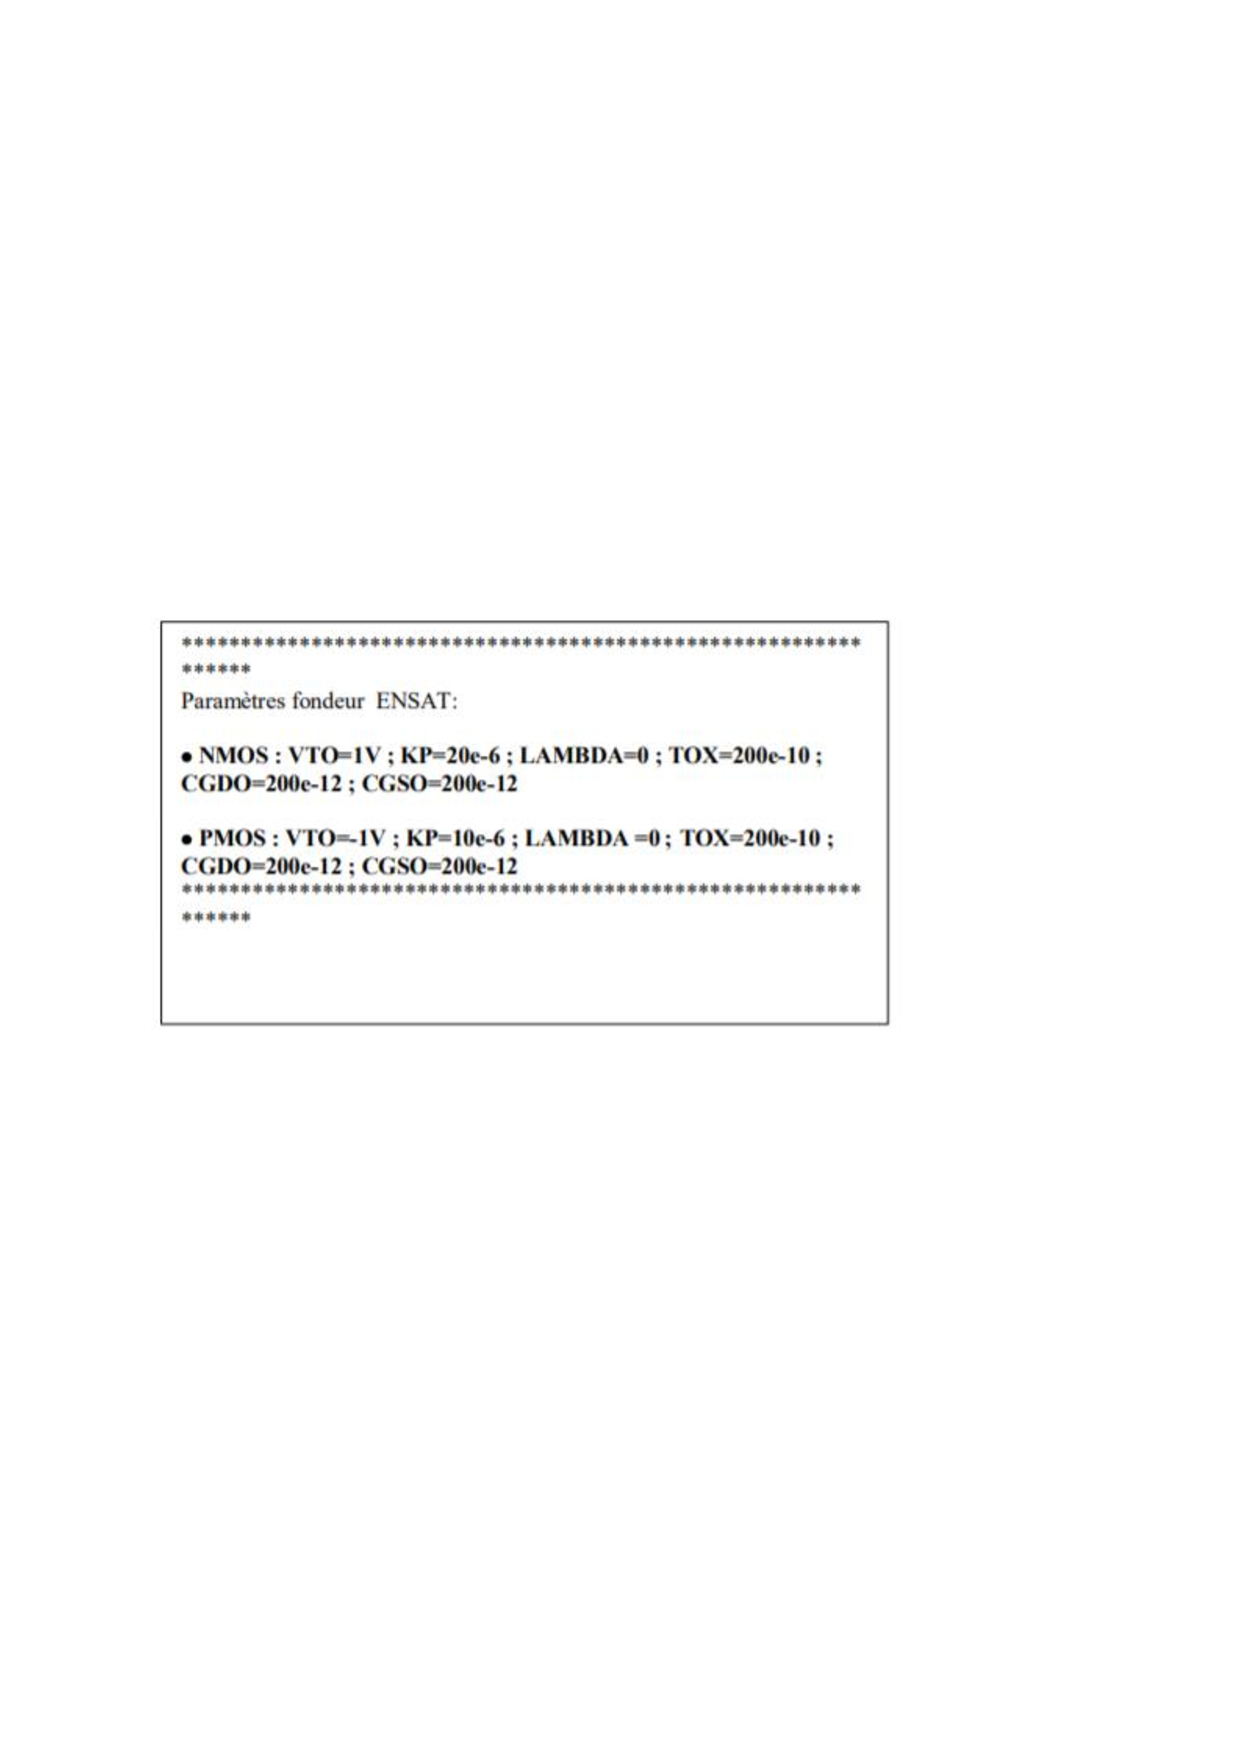
\includegraphics[width=0.45\textwidth]{Desing_Kit_ENSA.pdf}
    \caption{Layout du transistor en technologie ENSAT.}
    \label{fig:layout_ensat}
\end{figure}

\begin{figure}[H]
    \centering
    \includegraphics[width=0.75\textwidth]{Relais}
    \caption{Extrait de la documentation du relais RT42405.}
    \label{fig:Datasheet_RT424005}
\end{figure}

\vspace{0.5em}
\noindent\textbf{Calcul du rapport $W/L$ :} 

Le transistor pilote un relais nécessitant un courant nominal de maintien $I_{DS} = 80\,\text{mA}$ (pire cas sous 5 V, d'après la documentation). La commande du microcontrôleur impose $V_{GS} = 3,3\,\text{V}$.

Afin de minimiser la puissance dissipée et de garantir que la tension d'alimentation profite quasi-intégralement au relais, nous imposons une très faible chute de tension à l'état passant : \textbf{$V_{DS} = 0,1\,\text{V}$}. 

Puisque $V_{DS} < V_{GS} - V_{TO}$ ($0,1\,\text{V} < 2,3\,\text{V}$), le transistor opère bien en régime linéaire (ohmique). L'équation du courant de drain s'écrit alors :
\begin{equation}
    I_{DS} = K_P \frac{W}{L} \left[ (V_{GS} - V_{TO})V_{DS} - \frac{V_{DS}^2}{2} \right]
\end{equation}

En injectant nos valeurs nominales :
\begin{align*}
    0{,}08 &= 20 \cdot 10^{-6} \cdot \frac{W}{L} \left[ (3{,}3 - 1) \cdot 0{,}1 - \frac{0{,}1^2}{2} \right] \\
    0{,}08 &= 20 \cdot 10^{-6} \cdot \frac{W}{L} \cdot [0{,}225] \\
    \frac{W}{L} &= \frac{0{,}08}{4{,}5 \cdot 10^{-6}} \approx \mathbf{17\,778}
\end{align*}

\vspace{0.5em}
\noindent\textbf{Choix géométriques :} \\
En fixant la longueur du canal à la valeur typique de la technologie (\textbf{$L = 1\,\mu\text{m}$}), nous en déduisons une largeur nominale nécessaire de \textbf{$W = 17\,778\,\mu\text{m}$}.

\subsection{Question 2 : Validation des calculs par simulation PSpice}

Afin de valider notre modèle théorique, la simulation PSpice a été divisée en deux étapes : la caractérisation intrinsèque du silicium pour observer les régimes de fonctionnement (DC Sweep), puis la validation globale du composant intégré dans son circuit de commande (Bias Point).

\subsubsection{Caractérisation intrinsèque du silicium (DC Sweep)}

Pour cette étape, le transistor ($W = 17\,778\,\mu\text{m}$, $L = 1\,\mu\text{m}$) est isolé de son circuit de commande. L'objectif est de tracer ses caractéristiques de sortie pour valider son comportement théorique.

\begin{figure}[H]
    \centering
    \begin{minipage}{0.48\textwidth}
        \centering
        \includegraphics[width=\linewidth]{circuit_on.png} 
        \caption{Montage de caractérisation ON}
        \label{fig:test_on}
    \end{minipage}\hfill
    \begin{minipage}{0.48\textwidth}
        \centering
        \includegraphics[width=\linewidth]{circuit_off.png}
        \caption{Montage de caractérisation OFF}
        \label{fig:test_off}
    \end{minipage}
\end{figure}

\textbf{1. État Passant (Régime Ohmique)} \\
Le montage de la Figure \ref{fig:test_on} permet d'effectuer un balayage de la tension de drain avec une commande de grille idéale fixée à 3,3 V.

\begin{figure}[H]
    \centering
    \includegraphics[width=0.8\textwidth]{ids_vds_on.png}
    \caption{Caractéristique de sortie $I_{DS} = f(V_{DS})$ pour $V_{GS} = 3,3$ V.}
    \label{fig:courbe_on}
\end{figure}

\textbf{Analyse :} La Figure \ref{fig:courbe_on} confirme les régimes de fonctionnement attendus. En deçà de 2,3 V, la courbe est quasi-linéaire (régime ohmique). Au-delà, le courant sature. Au point de fonctionnement nominal (80 mA), la tension de drain n'est que de 101,4 mV. Cette valeur confirme que le transistor opère profondément en régime ohmique. La résistance à l'état passant est :
\begin{equation}
    R_{DS(on)} = \frac{V_{DS}}{I_{DS}} = \frac{0{,}1014\,\text{V}}{0{,}080\,\text{A}} \approx 1{,}26\,\Omega
\end{equation}

\textbf{2. État Bloqué (Régime de Coupure)} \\
La grille est ensuite portée à 0 V (Figure \ref{fig:test_off}).

\begin{figure}[H]
    \centering
    \includegraphics[width=0.8\textwidth]{ids_vds_off.png}
    \caption{Caractéristique de blocage $I_{DS} = f(V_{DS})$ pour $V_{GS} = 0$ V.}
    \label{fig:courbe_off}
\end{figure}

\textbf{Analyse :} La Figure \ref{fig:courbe_off} illustre l'excellente isolation du canal. Même sous une tension de drain maximale de 5 V, le courant de fuite est limité à 5,01 pA. Le composant agit comme un interrupteur ouvert quasi-idéal.

\subsubsection{Validation globale du circuit de commande (Bias Point)}

Le transistor est ensuite réinséré dans le circuit complet (Conception 1), incluant le pont diviseur et la charge. Une analyse statique du point de polarisation (\textit{Bias Point}) détermine les valeurs réelles d'équilibre du système.

\begin{figure}[H]
    \centering
    \begin{minipage}{0.5\textwidth}
        \centering
        \includegraphics[width=\linewidth]{schema_test_on.png} 
        \caption{Bias Point à l'état ON ($V_{uc} = 3,3$ V)}
        \label{fig:bias_on}
    \end{minipage}\hfill
    \begin{minipage}{0.5\textwidth}
        \centering
        \includegraphics[width=\linewidth]{schema_test_off.png}
        \caption{Bias Point à l'état OFF ($V_{uc} = 0$ V)}
        \label{fig:bias_off}
    \end{minipage}
\end{figure}

\textbf{Analyse du système intégré :}
\begin{itemize}
    \item \textbf{À l'activation (Figure \ref{fig:bias_on}) :} La tension de grille est légèrement atténuée par le réseau résistif d'entrée (3,229 V). La géométrie $W$ retenue permet d'assurer une faible chute de tension (102 mV) pour un courant traversant de 79 mA, garantissant le maintien magnétique du relais.
    \item \textbf{À l'extinction (Figure \ref{fig:bias_off}) :} La commande bascule à 0 V. Le courant est interrompu (5,01 pA) et le transistor bloque l'intégralité de la tension d'alimentation (5 V) en toute sécurité.
\end{itemize}

\subsection{Question 3 : Topologie et Layout sous Microwind}

Nous faisons face, lors de cette dernière étape, à une contrainte topologique majeure. Dessiner un ruban de silicium de $17.8\text{ mm}$ de large en une seule ligne droite est physiquement impensable ; cela génèrerait une puce filiforme et excessivement fragile.

Pour intégrer une telle largeur géante dans un espace carré et compact, la solution architecturale réside dans le dessin d'un transistor \textcolor{mainblue}{\textbf{"en peigne"}} (transistor interdigité ou \textit{multi-fingers}). Cette technique consiste à scinder le canal en une multitude de petits transistors placés en parallèle, partageant intelligemment leurs puits de Source et de Drain.

Si nous fixons la largeur d'un seul "doigt" de grille à $W_{doigt} = 50\ \mu\text{m}$, le nombre de doigts nécessaires se calcule simplement :
\begin{equation*}
    \text{Nombre de doigts} = \frac{W_{total}}{W_{doigt}} = \frac{17778}{50} \approx \textcolor{marron}{\mathbf{356 \text{ doigts}}}
\end{equation*}

Grâce à l'outil \textit{MOS Generator} de Microwind, nous avons pu compiler cette matrice. Le résultat, visible ci-dessous, montre l'enchevêtrement complexe du polysilicium (grille) et des diffusions actives. Notre "select Foundry" est  \textbf{cmos06.rul} 


\begin{figure}[H]
    \centering
     \includegraphics[width=1\textwidth]{Microwind.png}
     \caption{Layout du NMOS de puissance en topologie multi-fingers (356 doigts).}
 \end{figure}

Cette topologie illustre parfaitement l'enjeu principal de l'électronique de puissance sur silicium : le gain en dissipation thermique et en chute de tension ($V_{DS}$ minimal) se paie inévitablement par un coût drastique en surface (Area) sur la puce.

% ==============================================================================
% CONCLUSION GÉNÉRALE
% ==============================================================================

\section*{Conclusion Générale}
\addcontentsline{toc}{section}{Conclusion Générale}

Ce Bureau d'Étude a permis de concevoir et de valider une interface de commutation de puissance à deux échelles : macroscopique (carte imprimée) et microscopique (silicium).

D'une part, la \textbf{Conception 1} a abouti à une solution matérielle sécurisée. L'intégration d'un optocoupleur et d'une diode de roue libre a garanti l'isolation galvanique et la protection absolue du microcontrôleur (3,3 V) face à la charge inductive.

D'autre part, la \textbf{Conception 2} a transposé cette problématique en technologie intégrée (\textbf{ENSAT}). L'exigence d'une très faible chute de tension à l'état passant ($V_{DS} \approx 0{,}1\text{ V}$) a mis en lumière le compromis surface/performance, résolu géométriquement par le tracé d'un transistor en peigne ($W = 17{,}8\text{ mm}$).

En définitive, les deux approches répondent rigoureusement au cahier des charges. Les résultats, validés par la simulation (PSpice) et le dessin topologique (Microwind), consolident notre maîtrise de la chaîne de conception électronique complète, du Front-end au Back-end.
\newpage


% ==============================================================================
% BIBLIOGRAPHIE (Références Fiches Composants DigiKey)
% ==============================================================================
\begin{thebibliography}{9}

\bibitem{yageo_r220} 
Yageo, \emph{Datasheet - Résistance CMS Thick Film 220 Ohms RC0805FR-07220RL}, Catalogue DigiKey, \\
\url{https://www.digikey.com/en/products/detail/yageo/RC0805FR-07220RL/727741}

\bibitem{yageo_r10k} 
Yageo, \emph{Datasheet - Résistance CMS Thick Film 10 kOhms RC0805FR-0710KL}, Catalogue DigiKey, \\
\url{https://www.digikey.com/en/products/detail/yageo/RC0805FR-0710KL/727535}

\bibitem{ir_mosfet} 
Infineon Technologies, \emph{Datasheet - Transistor MOSFET N-Channel IRLML2502TRPBF}, Catalogue DigiKey, \\
\url{https://www.digikey.com/en/products/detail/infineon-technologies/IRLML2502TRPBF/811439}

\bibitem{goodwork_diode} 
GK(GOODWORK), \emph{Datasheet - Diode de Commutation Rapide SOD-323 1N4148WTR-ND}, Catalogue DigiKey, \\
\url{https://www.digikey.com/en/products/detail/goodwork/1N4148W/29292003}

\bibitem{liteon_opto} 
Lite-On Electronics, \emph{Datasheet - Optocoupleur Phototransistor SOP-4 LTV-817S (Réf: 160-1367-5-ND)}, Catalogue DigiKey, \\
\url{https://www.digikey.com/en/products/detail/liteon/LTV-817S/385837}

\bibitem{te_relais} 
TE Connectivity Potter \& Brumfield Relays, \emph{Datasheet - Relais Électromécanique RT2 RT424005}, Catalogue DigiKey, \\
\url{https://www.digikey.com/en/products/detail/wee/RT424005/24883690}

\bibitem{dfrobot_pcb} 
DFRobot, \emph{Fiche Spécification Technique - Prototyping Board Double Face FR4 FIT0203}, Catalogue DigiKey, \\
\url{https://www.digikey.com/en/products/detail/dfrobot/FIT0203/6588423}

\bibitem{sparkfun_sot23} 
SparkFun Electronics, \emph{Fiche Technique - Adaptateur CMS SOT-23 vers DIP BOB-00717}, Catalogue DigiKey, \\
\url{https://www.digikey.com/en/products/detail/sparkfun-electronics/00717/5318740}

\end{thebibliography}

\end{document}